

\section{Reinforcement Learning Framework}

\subsection{Agent-Environment Interaction}

Reinforcement Learning (RL) formalizes the problem of learning optimal behavior through trial-and-error interaction with an environment (Figure~\ref{fig:rl_framework}).

\begin{figure}[htbp]
    \centering
    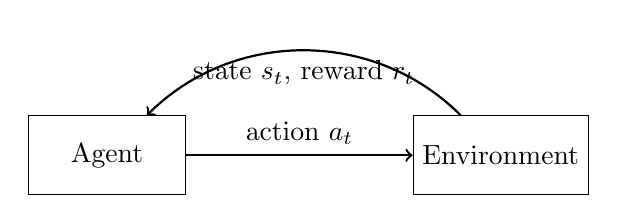
\begin{tikzpicture}[node distance=3cm, auto]
        \node [draw, rectangle, minimum width=2cm, minimum height=1cm] (agent) {Agent};
        \node [draw, rectangle, minimum width=2cm, minimum height=1cm, right of=agent, node distance=5cm] (env) {Environment};
        
        \draw[->, thick] (agent) -- node[above] {action $a_t$} (env);
        \draw[->, thick] (env) to [bend right=45] node[below] {state $s_t$, reward $r_t$} (agent);
    \end{tikzpicture}
    \caption{Agent-environment interaction in reinforcement learning}
    \label{fig:rl_framework}
\end{figure}

The framework consists of several key components. The \textbf{Agent} is the controller implemented using DDPG or TD3 neural networks, while the \textbf{Environment} is the hybrid DFIG-PV power system being controlled. The \textbf{State $s_t$} represents system measurements at time $t$, and the \textbf{Action $a_t$} comprises control voltages applied to converters. The \textbf{Reward $r_t$} is a scalar feedback signal indicating performance, and the \textbf{Policy $\pi$} defines the mapping from states to actions.

\subsection{Markov Decision Process (MDP)}

The RL problem is formally defined as a Markov Decision Process:

\begin{definition}[Markov Decision Process]
An MDP is a tuple $\mathcal{M} = (\mathcal{S}, \mathcal{A}, P, R, \gamma)$ where:
\begin{itemize}
    \item $\mathcal{S}$ is the state space
    \item $\mathcal{A}$ is the action space
    \item $P(s_{t+1}|s_t, a_t)$ is the state transition probability
    \item $R(s_t, a_t)$ is the reward function
    \item $\gamma \in [0,1]$ is the discount factor
\end{itemize}
\end{definition}

\textbf{Markov Property:}
\begin{equation}
P(s_{t+1}|s_t, a_t, s_{t-1}, a_{t-1}, \ldots, s_0, a_0) = P(s_{t+1}|s_t, a_t)
\end{equation}

\section{Policy and Value Functions}

\subsection{Policy}

A policy $\pi$ defines the agent's behavior. For deterministic policies (used in DDPG and TD3):
\begin{equation}
a = \pi(s)
\end{equation}

The goal is to find the optimal policy:
\begin{equation}
\pi^* = \argmax_\pi \EE\left[\sum_{t=0}^{\infty} \gamma^t r_t \Big| \pi\right]
\end{equation}

\subsection{Value Functions}

\begin{definition}[Action-Value Function]
The Q-function is the expected return starting from state $s$, taking action $a$:
\begin{equation}
Q^\pi(s,a) = \EE_\pi\left[\sum_{k=0}^{\infty} \gamma^k r_{t+k} \Big| s_t = s, a_t = a\right]
\end{equation}
\end{definition}

\subsection{Bellman Equation}

The Q-function satisfies the Bellman optimality equation:
\begin{equation}
Q^*(s,a) = \EE_{s'}\left[r + \gamma \max_{a'} Q^*(s',a')\right]
\label{eq:bellman}
\end{equation}

\section{Actor-Critic Architecture}

Actor-critic methods combine two components: the \textbf{Actor} learns the policy $\pi_\theta(s)$ parameterized by $\theta$, while the \textbf{Critic} learns the value function $Q_\phi(s,a)$ parameterized by $\phi$ (Figure~\ref{fig:actor_critic_general}).

\begin{figure}[htbp]
    \centering
    \includegraphics[width=0.7\textwidth]{images/Actor_Critic_Diagram.png}
    \caption{General actor-critic architecture showing the interaction between policy network (actor) and value network (critic) in reinforcement learning-based control}
    \label{fig:actor_critic_general}
\end{figure}

\subsection{Deterministic Policy Gradient}

For deterministic policies $a = \mu_\theta(s)$, the policy gradient is:
\begin{equation}
\nabla_\theta J(\theta) = \EE_{s \sim \rho^\mu}\left[\nabla_\theta \mu_\theta(s) \nabla_a Q(s,a)|_{a=\mu_\theta(s)}\right]
\label{eq:dpg}
\end{equation}

This is the foundation of DDPG and TD3 \cite{Fathollahi2024,Yakout2025}. Recent applications of deep deterministic policy gradient methods in power systems have demonstrated superior performance compared to traditional control approaches, particularly for adaptive voltage regulation and transient stability enhancement in grid-connected renewable energy systems.

\section{Experience Replay}

Experience replay stores transitions in a buffer $\mathcal{B}$:
\begin{equation}
\mathcal{B} = \{(s_t, a_t, r_t, s_{t+1})\}_{t=1:T}
\end{equation}

Training uses random minibatches to break temporal correlations and improve sample efficiency.

\section{Target Networks}

Target networks provide stable regression targets. Separate target networks with parameters $\theta'$ and $\phi'$ are slowly updated:
\begin{align}
\theta' &\leftarrow \tau \theta + (1-\tau)\theta' \\
\phi' &\leftarrow \tau \phi + (1-\tau)\phi'
\end{align}
where $\tau \ll 1$ (typically 0.001).

Target Q-value:
\begin{equation}
y_t = r_t + \gamma Q_{\phi'}(s_{t+1}, \mu_{\theta'}(s_{t+1}))
\end{equation}

\section{Twin-Delayed Deep Deterministic Policy Gradient (TD3)}

\subsection{TD3 Algorithm Overview}

Twin-Delayed DDPG (TD3) addresses critical overestimation bias in actor-critic methods through three key innovations: twin critic networks, delayed policy updates, and target policy smoothing \cite{Zholtayev2024,Muktiadji2024,Pandey2025TD3}. Recent applications in renewable energy systems demonstrate TD3's superior robustness and performance compared to baseline DDPG implementations, particularly for solar PV-integrated DFIG wind energy systems \cite{Pandey2025TD3}.

\textbf{Key TD3 Innovations:}

\begin{enumerate}
    \item \textbf{Twin Critic Networks:} Maintains two independent Q-networks $Q_{\phi_1}$ and $Q_{\phi_2}$, using the minimum value for policy updates to reduce overestimation bias

    \item \textbf{Delayed Policy Updates:} Updates the actor network less frequently than critics (typically every 2nd iteration) to allow Q-values to stabilize before policy refinement

    \item \textbf{Target Policy Smoothing:} Adds bounded noise to target actions during training to prevent exploitation of Q-function errors
\end{enumerate}

The TD3 architecture with twin critic networks is illustrated in Figure~\ref{fig:td3_actor_critic}, which shows how the dual critic approach mitigates overestimation bias by taking the minimum Q-value estimate for policy updates.

\begin{figure}[htbp]
    \centering
    \includegraphics[width=0.6\textwidth]{images/TD3ActorCritic.png}
    \caption{TD3 actor-critic network architecture with twin critic networks ($Q_1$ and $Q_2$) for improved value estimation and reduced overestimation bias in DFIG-Solar PV hybrid system control}
    \label{fig:td3_actor_critic}
\end{figure}

\subsection{TD3 Applications in Renewable Energy Systems}

Recent research demonstrates TD3's effectiveness across multiple renewable energy applications:

\textbf{Wind Energy Control:} TD3 has been successfully applied to maximum power point tracking (MPPT) in wind turbine systems \cite{Zholtayev2024}, showing superior robustness to parameter variations compared to model-based feedback linearization methods. The model-free nature of TD3 eliminates the need for accurate system models, making it particularly valuable for DFIG systems with complex nonlinear dynamics.

\textbf{DC Microgrid Power Electronics:} For boost converter control in DC microgrids \cite{Muktiadji2024}, TD3 outperforms particle swarm optimization (PSO), genetic algorithms (GA), and conventional PI controllers with significantly reduced steady-state error and faster transient response times. This application is directly relevant to solar PV integration where DC-DC converters regulate the DC-link voltage.

\textbf{Virtual Power Plant Management:} In large-scale renewable energy aggregation systems \cite{Hu2025VPP}, TD3-based energy management strategies achieve 84.71\% and 94.39\% higher mean reward compared to TD3-battery and DDPG-EV baselines, with 16.7\% cost reduction and 89.45\% reduction in microturbine output. These results demonstrate TD3's scalability and multi-objective optimization capabilities for complex hybrid renewable systems.

\section{Deep Deterministic Policy Gradient (DDPG) Applications}

\subsection{DDPG for Grid Stability and Voltage Control}

DDPG has emerged as a powerful tool for grid-connected renewable energy systems, particularly for addressing stability challenges and power optimization in hybrid solar PV-integrated DFIG systems \cite{Pandey2025DDPG}:

\textbf{Rotor Angle Stability Enhancement:} DDPG-based power system stabilizers \cite{Yakout2025} demonstrate superior performance over multi-band PSS and conventional lead PSS controllers for transient stability improvement. Validation on single-machine infinite-bus (SMIB), Kundur 4-machine, and IEEE 39-bus systems confirms DDPG's effectiveness for maintaining synchronous stability in grids with high renewable penetration—critical for DFIG wind systems during grid disturbances.

\textbf{Adaptive Voltage Regulation:} DDPG-based synergetic control for synchronous generator excitation systems \cite{Fathollahi2024} achieves fast adaptive voltage regulation and stability improvement under various disturbances. This approach is highly relevant for hybrid DFIG-PV systems that must maintain grid voltage within IEEE 1547 limits (±5\%) during rapid solar irradiance and wind speed variations.

\subsection{Comparative Analysis: DDPG vs. TD3}

While both algorithms share the deterministic policy gradient foundation, TD3's three key innovations address DDPG's primary weaknesses. TD3's twin critics reduce Q-value overestimation, leading to more conservative and stable policy learning. Delayed policy updates prevent rapid policy changes based on noisy Q-estimates, reducing policy oscillation. Target policy smoothing improves generalization and reduces sensitivity to hyperparameter choices, enhancing overall robustness.

However, DDPG remains computationally simpler during training and may be preferable for real-time adaptive control scenarios where training overhead is critical.

\section{Advanced Actor-Critic Methods for Renewable Energy}

\subsection{Soft Actor-Critic (SAC) for Microgrid Optimization}

Soft Actor-Critic (SAC) extends actor-critic methods by maximizing both expected reward and policy entropy, promoting exploration and robustness \cite{Yu2024,Liang2024}. For microgrid energy management, improved SAC algorithms achieve 51.20\%, 52.38\%, and 13.43\% profit increases over DQN, SARSA, and PPO respectively, demonstrating superior economic optimization capabilities.

SAC's application to integrated energy systems with electricity, heat, and hydrogen storage \cite{Liang2024} showcases model-free control for multi-energy systems with complex energy coupling—relevant for future DFIG-PV systems integrated with energy storage and hydrogen production facilities.

\subsection{Multi-Objective Deep RL for Wind Turbines}

Actor-critic deep RL enables multi-objective optimization beyond simple MPPT \cite{Frutos2025}. For 2.3 MW wind turbines, deep RL balances power maximization with operational constraints such as noise mitigation, mechanical stress reduction, and grid code compliance. This multi-objective capability is essential for commercial DFIG installations where regulatory compliance, equipment lifespan, and power quality must be simultaneously optimized.

\subsection{Quantum-Inspired Actor-Critic Methods}

Emerging quantum-inspired approaches \cite{Shen2024} demonstrate improved performance for frequency regulation in renewable-dominated microgrids. Quantum-inspired maximum entropy actor-critic (QISMEAC) algorithms outperform standard SAC and DDPG for handling renewable intermittency, offering potential pathways for next-generation control systems capable of managing high-penetration renewable grids with minimal frequency deviations (±0.2 Hz IEEE 1547 requirement).

\section{Model-Free Control Advantages for Hybrid Systems}

The fundamental advantage of deep reinforcement learning for DFIG-PV hybrid systems lies in their model-free nature. Unlike model predictive control (MPC), DRL directly learns optimal policies from nonlinear system dynamics without requiring linearization or explicit system models. DRL controllers trained with diverse operating conditions demonstrate robust performance across parameter uncertainties inherent in renewable energy systems including turbine inertia variations, PV array degradation, and grid impedance changes. Actor-critic methods naturally handle continuous control signals such as rotor-side converter voltages and grid-side converter modulation indices without discretization artifacts. Finally, reward function design enables simultaneous optimization of multiple conflicting objectives including power maximization, grid stability, THD minimization, and fault ride-through capability.

These advantages position TD3 and DDPG as promising alternatives to traditional PI/PID cascades and model-based controllers for next-generation hybrid renewable energy systems.